% =============================================================================
% Project : THE_PHILOSOPHY_OF_VIABILITY
% Book    : Book I — Ontology of Viability
% Book ID : VS.B01
%
% File    : 4_ASSETS/illustrations/VS.B01.P01.C03.S07.SS04.P003.IL01.numerical_singularity_uniqueness_and_aggregate.tex
%
% Asset:
%   Illustration IL01 — Numerical Singularity, Uniqueness,
%   and Aggregate
%
% Purpose :
%   To illustrate three different descriptions:
%   one selected item within a plurality, one item unique
%   under a specified criterion, and one collection counted
%   as a unit despite its multiple members.
%
% =============================================================================

\begin{figure}[htbp]
\centering

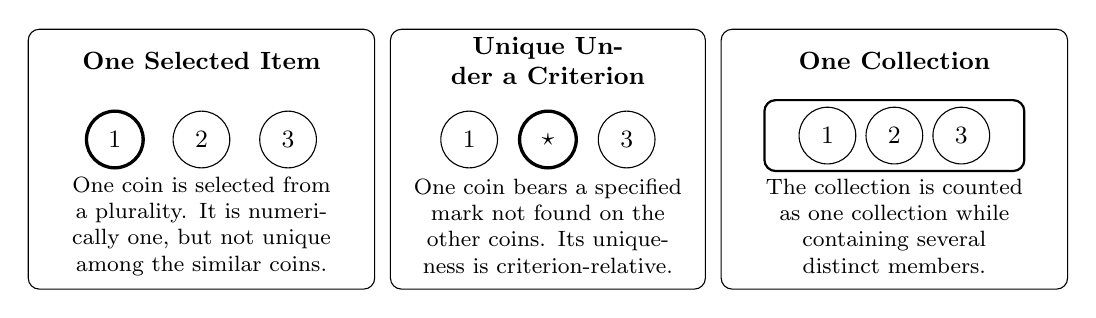
\begin{tikzpicture}[
    coin/.style={
        draw,
        circle,
        minimum size=0.72cm,
        inner sep=1pt,
        align=center,
        font=\small
    },
    panel/.style={
        draw,
        rounded corners,
        minimum width=4.25cm,
        minimum height=3.25cm
    },
    paneltitle/.style={
        font=\small\bfseries,
        align=center,
        text width=3.8cm
    },
    explanation/.style={
        font=\footnotesize,
        align=center,
        text width=3.8cm
    }
]

% Panel A: One selected item, not unique
\draw[panel] (-6.6,-1.65) rectangle (-2.2,1.65);

\node[paneltitle] at (-4.4,1.25) {
    One Selected Item
};

\node[coin, very thick] at (-5.5,0.25) {1};
\node[coin] at (-4.4,0.25) {2};
\node[coin] at (-3.3,0.25) {3};

\node[explanation] at (-4.4,-0.85) {
    One coin is selected from a plurality.
    It is numerically one, but not unique
    among the similar coins.
};

% Panel B: Unique under a criterion
\draw[panel] (-2.0,-1.65) rectangle (2.0,1.65);

\node[paneltitle] at (0,1.25) {
    Unique Under a Criterion
};

\node[coin] at (-1.0,0.25) {1};
\node[coin, very thick] at (0,0.25) {$\star$};
\node[coin] at (1.0,0.25) {3};

\node[explanation] at (0,-0.85) {
    One coin bears a specified mark
    not found on the other coins.
    Its uniqueness is criterion-relative.
};

% Panel C: One collection, multiple members
\draw[panel] (2.2,-1.65) rectangle (6.6,1.65);

\node[paneltitle] at (4.4,1.25) {
    One Collection
};

\draw[rounded corners, thick]
    (2.75,-0.15) rectangle (6.05,0.75);

\node[coin] at (3.55,0.3) {1};
\node[coin] at (4.4,0.3) {2};
\node[coin] at (5.25,0.3) {3};

\node[explanation] at (4.4,-0.85) {
    The collection is counted as one
    collection while containing several
    distinct members.
};

\end{tikzpicture}

\caption{Numerical Singularity, Uniqueness, and the Unity of a Collection}
\label{fig:numerical-singularity-uniqueness-and-aggregate}
\end{figure}

% =============================================================================
% END OF ILLUSTRATION IL01
% =============================================================================